\appendix
\chapter{Statistics} \label{ch:appendix_statistic}
\section{Temporal Statistics and Deviation} \label{sec:all_stats}
%%% ALL LOCAL STATISTICS FOR VARIABLES 
%% TEMPERATURE
\begin{figure}[ht]
    \centering
    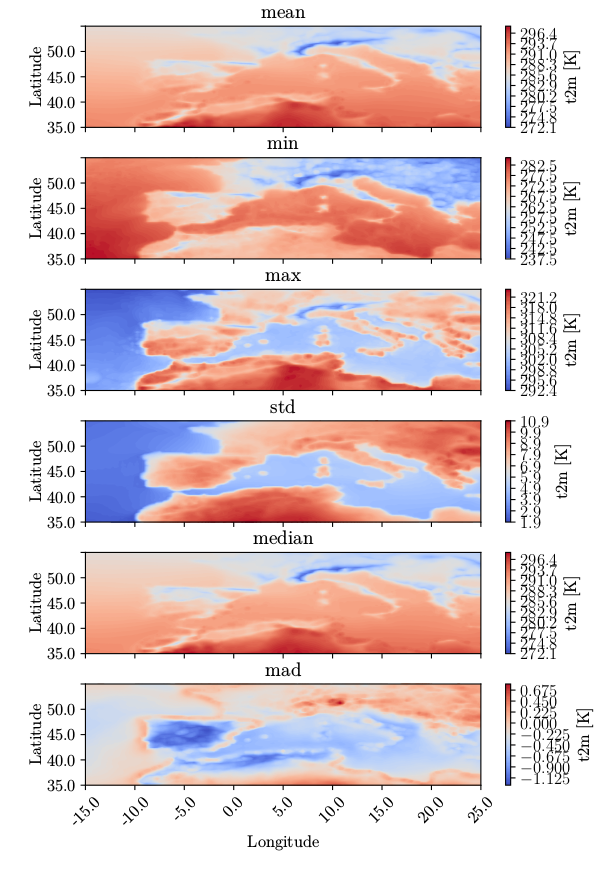
\includegraphics[scale=0.9]{python_figs/all_stat_variable_t2m.png}
    \caption{Contour plot showing the local (pixel) statistics for temperature.}
    \label{fig:all_stats_t2m}
\end{figure}
%% SURFACE PRESSURE 
\begin{figure}[ht]
    \centering
    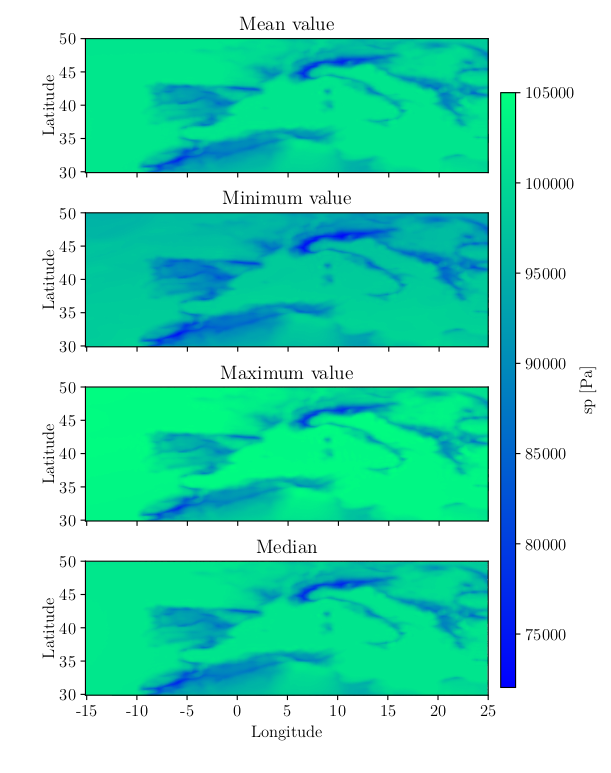
\includegraphics{python_figs/all_stat_variable_sp.png}
    \caption{Contour plot showing the local (pixel) statistics for surface pressure.}
    \label{fig:all_stats_sp}
\end{figure}
%% RELATIVE HUMIDITY 
\begin{figure}[ht]
    \centering
    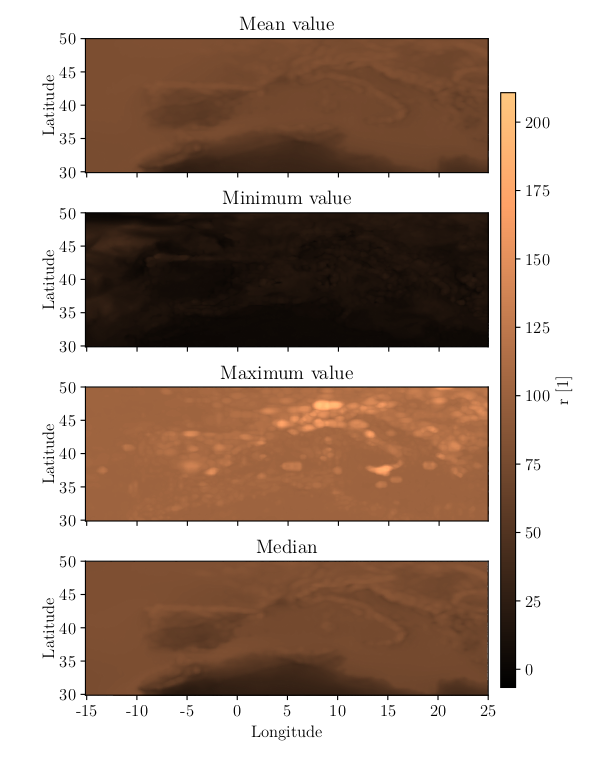
\includegraphics{python_figs/all_stat_variable_r.png}
    \caption{Contour plot showing the local (pixel) statistics for relative humidity.}
    \label{fig:all_stats_r}
\end{figure}
%% SPECIFIC HUMIDITY 
\begin{figure}[ht]
    \centering
    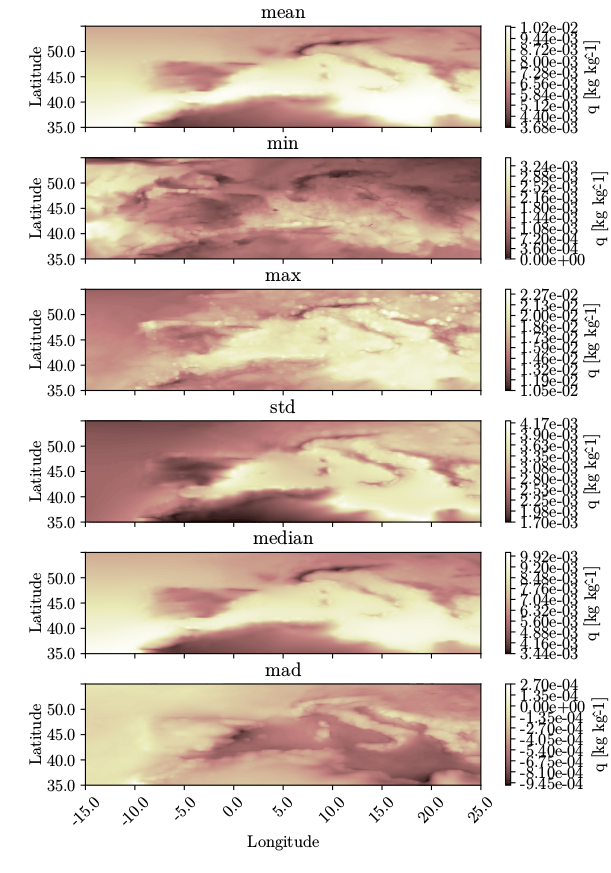
\includegraphics{python_figs/all_stat_variable_q.png}
    \caption{Contour plot showing the local (pixel) statistics for specific humidity.}
    \label{fig:all_stats_q}
\end{figure}
\cleardoublepage
\section{Temporal Statistics Deviations} \label{sec:all_stats_deviation}
\begin{figure}[ht]
    \centering
    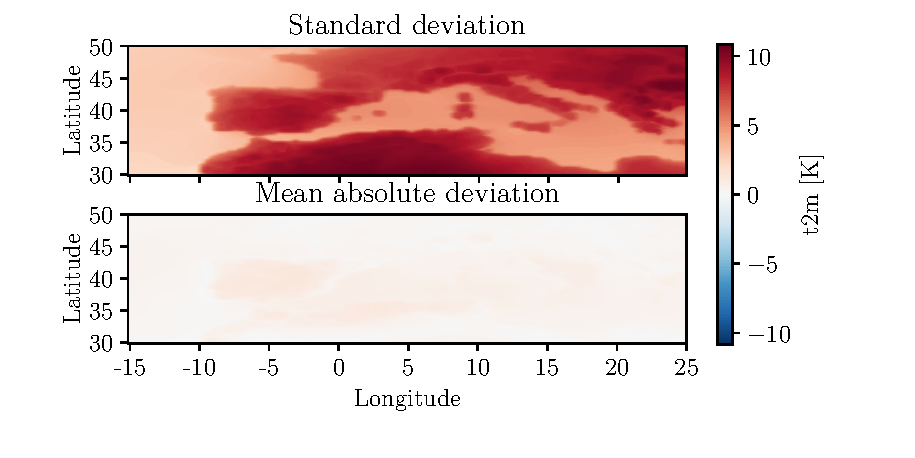
\includegraphics{python_figs/DEVIATION_all_stat_variable_t2m.pdf}
    \caption{Deviations in two meter temperature, $t_2m$.}
    \label{fig:deviation_t2m}
\end{figure}
\begin{figure}[ht]
    \centering
    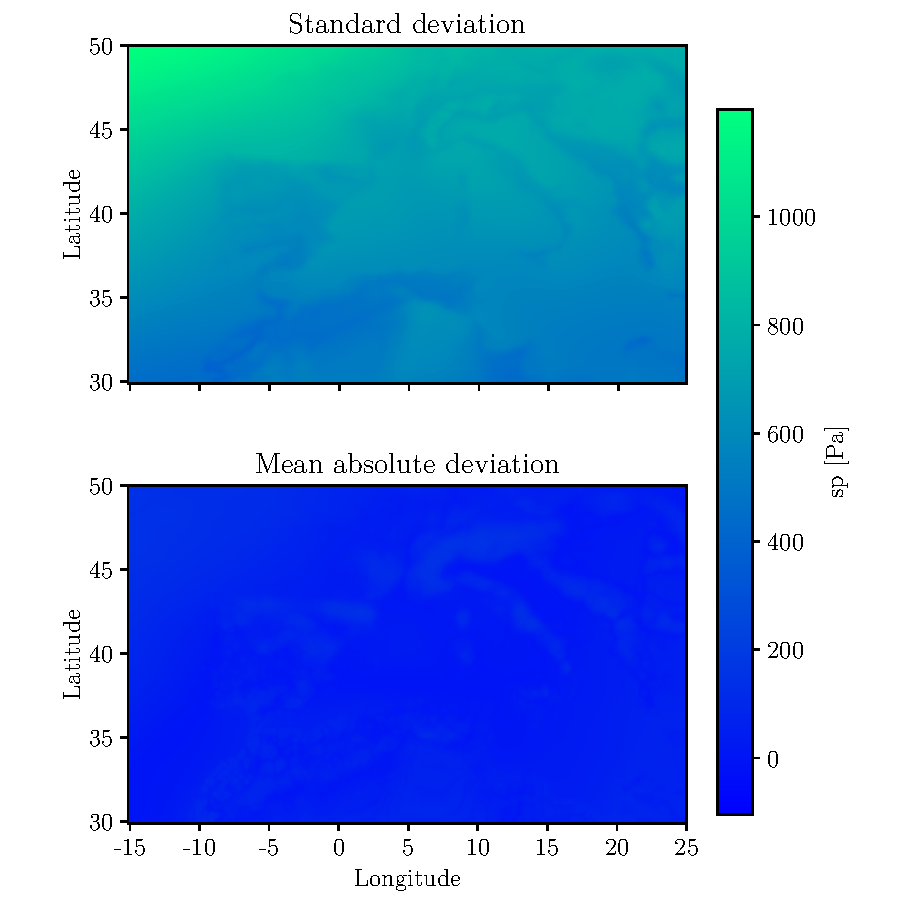
\includegraphics{python_figs/DEVIATION_all_stat_variable_sp.pdf}
    \caption{Deviations in surface pressure, sp.}
    \label{fig:deviation_sp}
\end{figure}
\begin{figure}[ht]
    \centering
    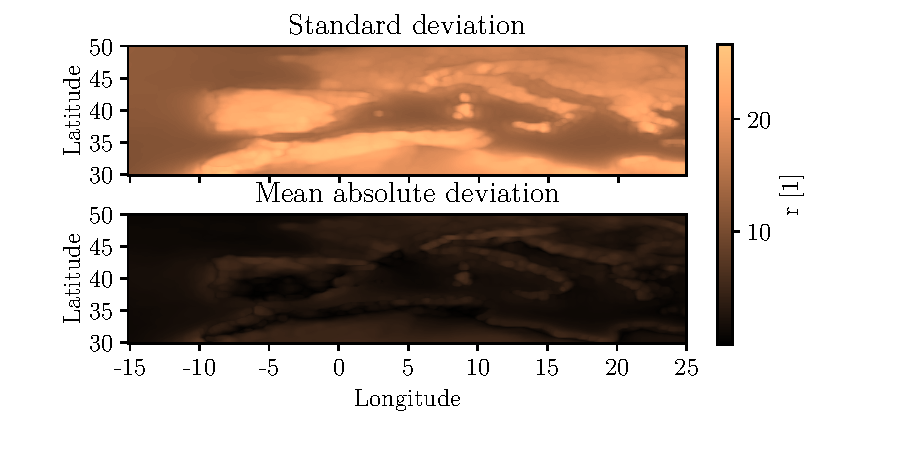
\includegraphics{python_figs/DEVIATION_all_stat_variable_r.pdf}
    \caption{Deviations in relative humidity, r.}
    \label{fig:deviation_r}
\end{figure}
\begin{figure}[ht]
    \centering
    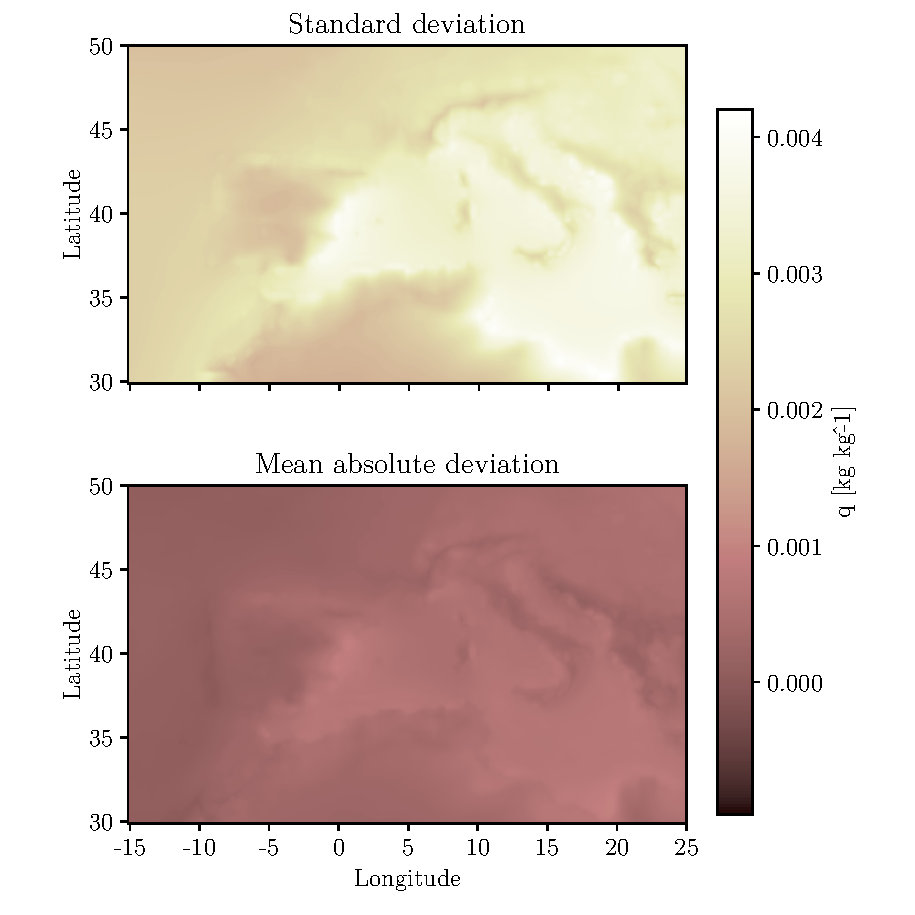
\includegraphics{python_figs/DEVIATION_all_stat_variable_q.pdf}
    \caption{Deviations in specific humidity, q.}
    \label{fig:deviation_q}
\end{figure}


\cleardoublepage
\chapter{Seasonal effects} \label{app:seasonal_plots}
\begin{figure}[ht]
    \centering
    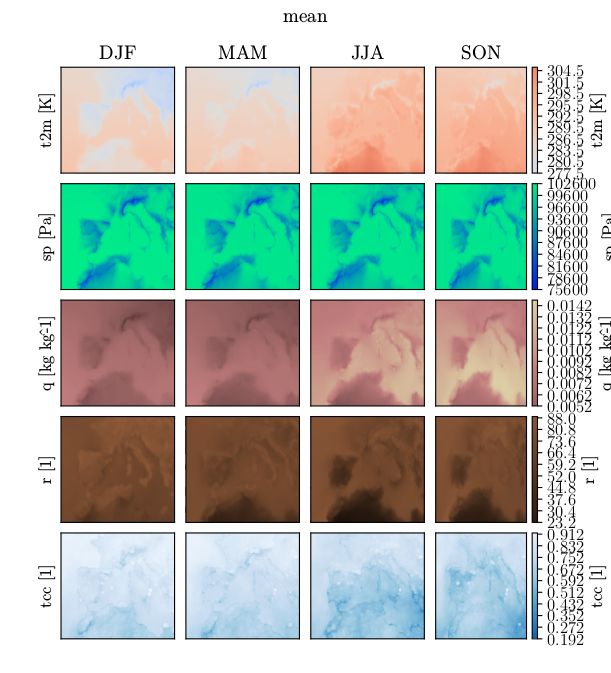
\includegraphics{python_figs/seasonal_mean_all_variables.png}
    \caption{Seasonal mean for all variables in \acrshort{ecc}.}
    \label{fig:seasonal_mean}
\end{figure}

\begin{figure}[ht]
    \centering
    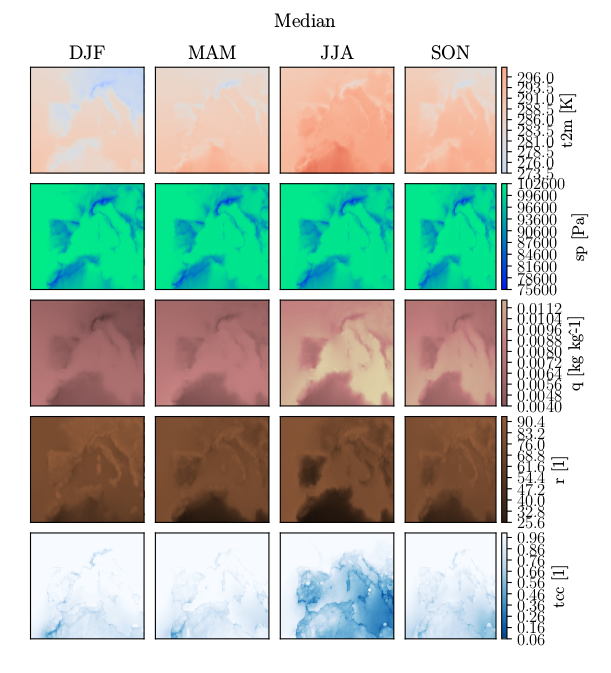
\includegraphics{python_figs/seasonal_median_all_variables.png}
    \caption{Seasonal median for all variables in \acrshort{ecc}.}
    \label{fig:seasonal_median}
\end{figure}

%\cleardoublepage
%\chapter{Time Evolution of \acrlong{cfc} } \label{app:timelapse}
%\begin{figure}[ht]
%    \centering
%    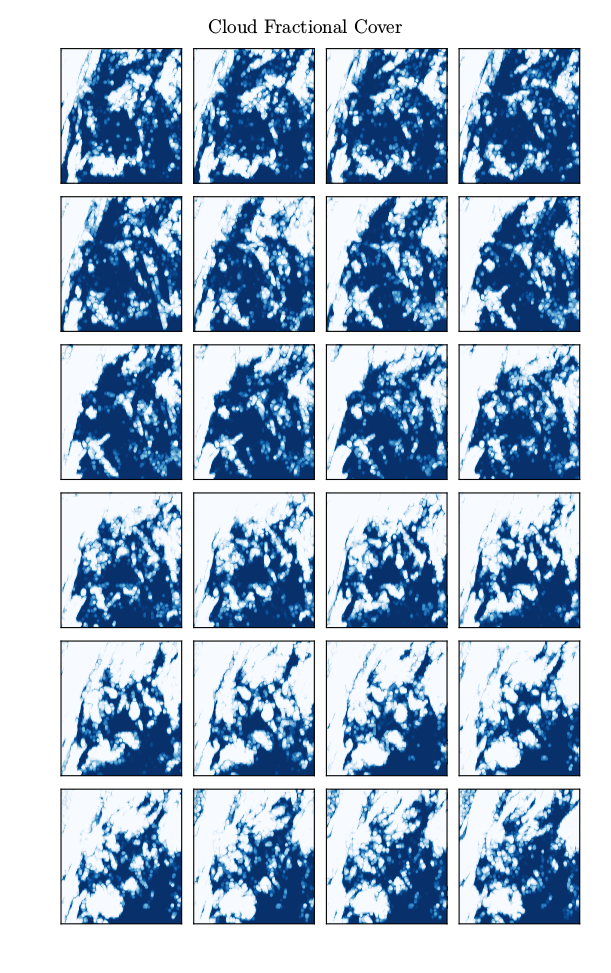
\includegraphics[scale=0.70]{python_figs/timelapse_cloud_cover_24hrs_from_2010-07-01.png}
%    \caption{Time evolution of cloud fractional cover 24 hours from July first 2010.}
%    \label{fig:time_lapse}
%\end{figure}

\cleardoublepage
\chapter{Series of First Weeks in 2012} \label{app:first_week}
%\addcontentsline{toc}{chapter}{Appendix D: Study 2012}
\begin{figure}[ht]
    \centering
    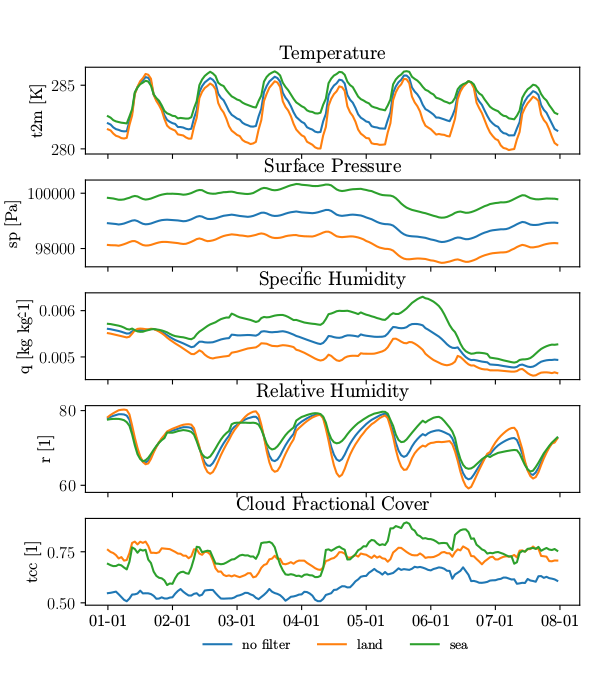
\includegraphics{python_figs/spatially_averaged_one_week_from_2012-01-01.png}
    \caption{\acrshort{ecc} variables first week January 2012.}
    \label{fig:jan12}
\end{figure}
\begin{figure}[ht]
    \centering
    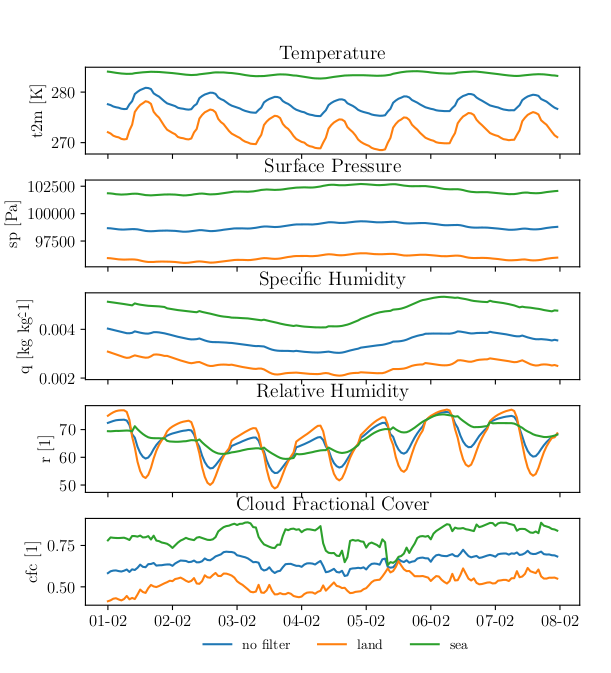
\includegraphics{python_figs/spatially_averaged_one_week_from_2012-02-01.png}
    \caption{\acrshort{ecc} variables first week February 2012.}
    \label{fig:feb12}
\end{figure}
\begin{figure}[ht]
    \centering
    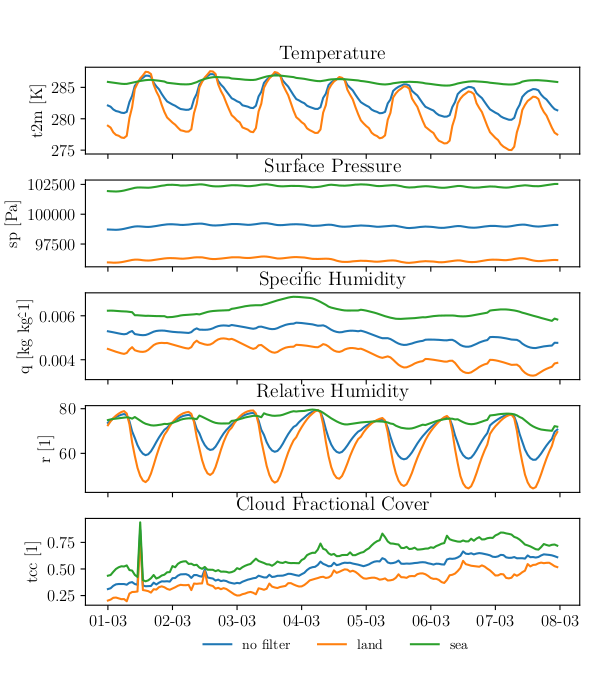
\includegraphics{python_figs/spatially_averaged_one_week_from_2012-03-01.png}
    \caption{\acrshort{ecc} variables first week March 2012.}
    \label{fig:mar12}
\end{figure}
\begin{figure}[ht]
    \centering
    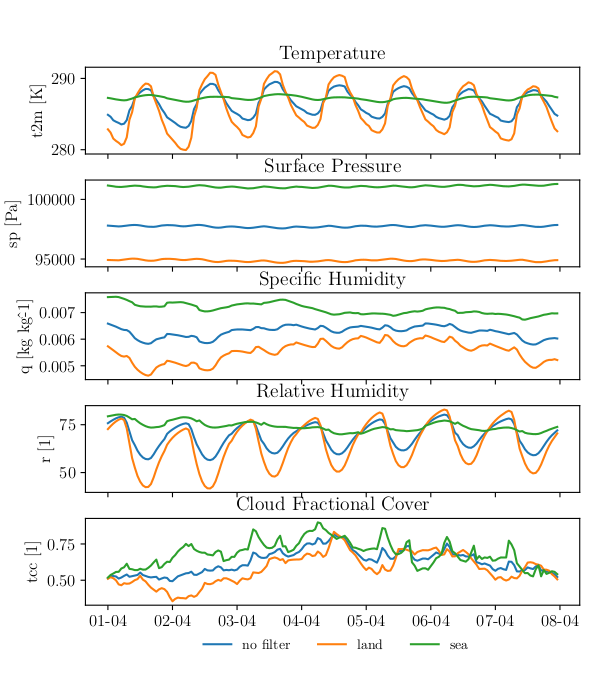
\includegraphics{python_figs/spatially_averaged_one_week_from_2012-04-01.png}
    \caption{\acrshort{ecc} variables first week April 2012.}
    \label{fig:april12}
\end{figure}
\begin{figure}[ht]
    \centering
    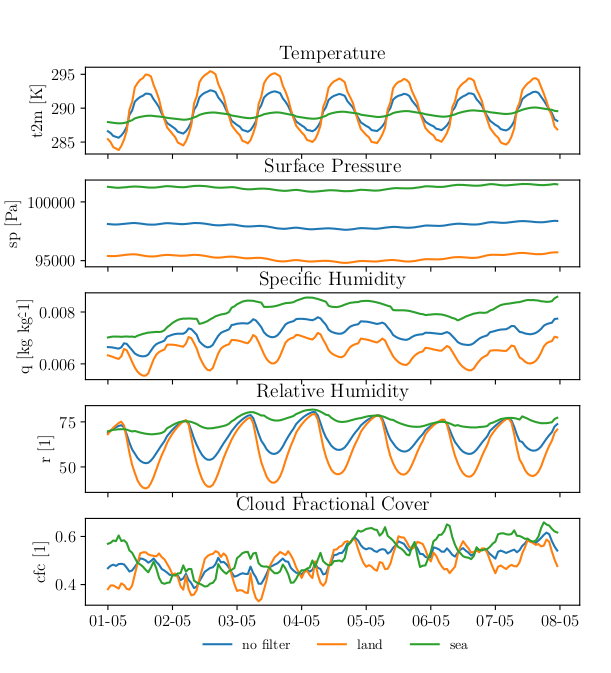
\includegraphics{python_figs/spatially_averaged_one_week_from_2012-05-01.png}
    \caption{\acrshort{ecc} variables first week May 2012.}
    \label{fig:may12}
\end{figure}
\begin{figure}[ht]
    \centering
    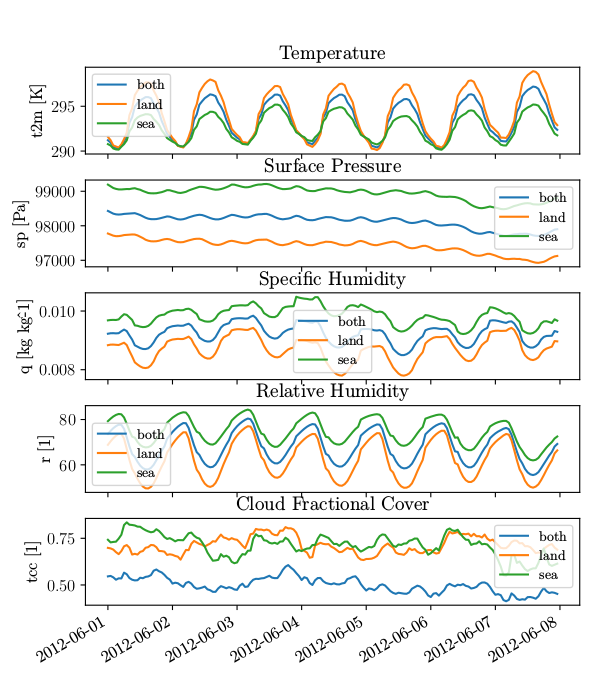
\includegraphics{python_figs/spatially_averaged_one_week_from_2012-06-01.png}
    \caption{\acrshort{ecc} variables first week June 2012.}
    \label{fig:jun12}
\end{figure}
\begin{figure}[ht]
    \centering
    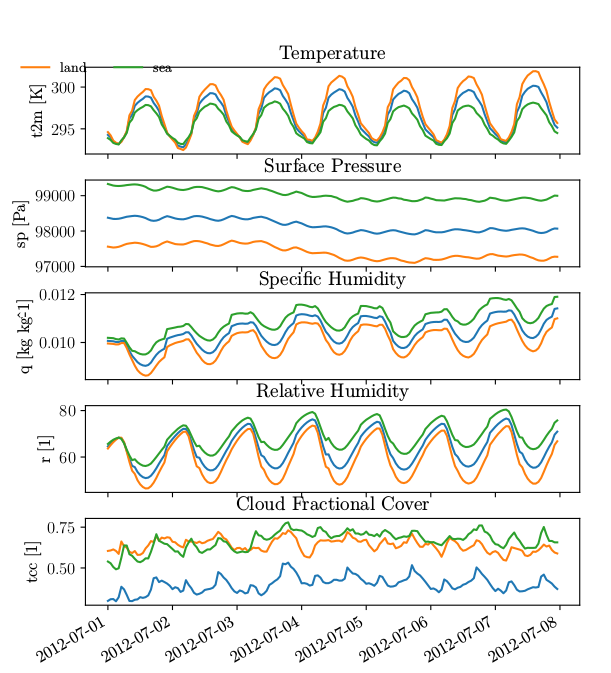
\includegraphics{python_figs/spatially_averaged_one_week_from_2012-07-01.png}
    \caption{\acrshort{ecc} variables first week July 2012.}
    \label{fig:jul12}
\end{figure}
\begin{figure}[ht]
    \centering
    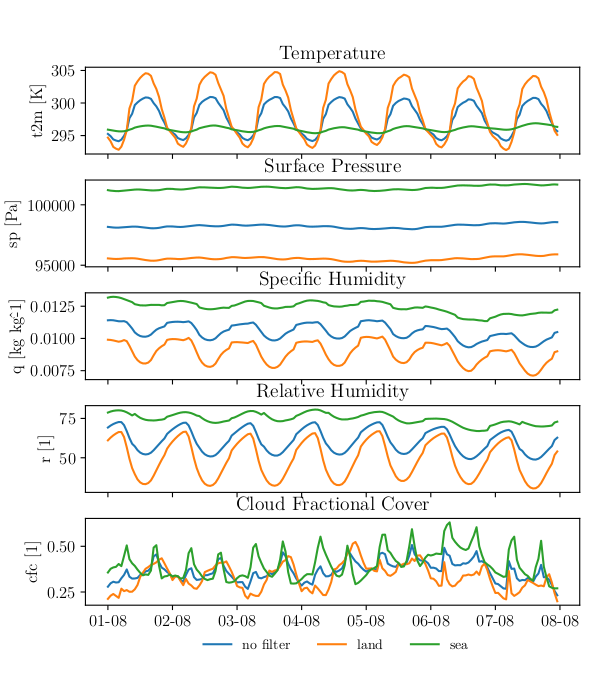
\includegraphics{python_figs/spatially_averaged_one_week_from_2012-08-01.png}
    \caption{\acrshort{ecc} variables first week August 2012.}
    \label{fig:aug12}
\end{figure}
% September is in the text
\begin{figure}[ht]
    \centering
    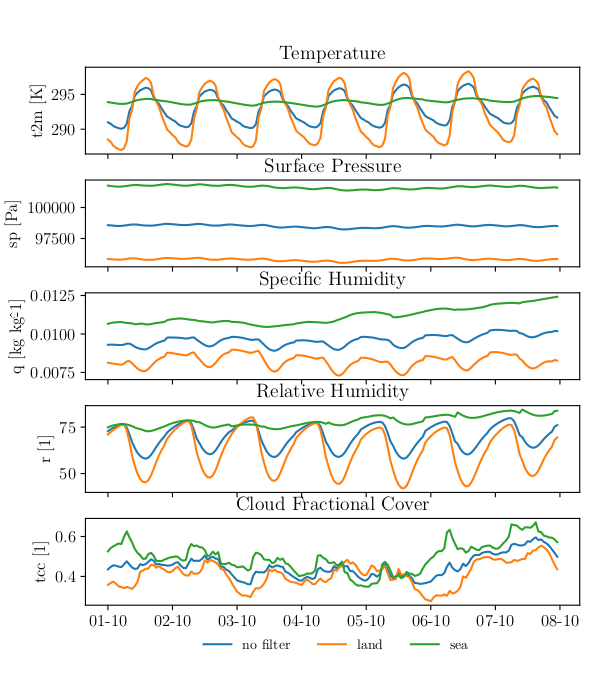
\includegraphics{python_figs/spatially_averaged_one_week_from_2012-10-01.png}
    \caption{\acrshort{ecc} variables first week October 2012.}
    \label{fig:oct12}
\end{figure}
\begin{figure}[ht]
    \centering
    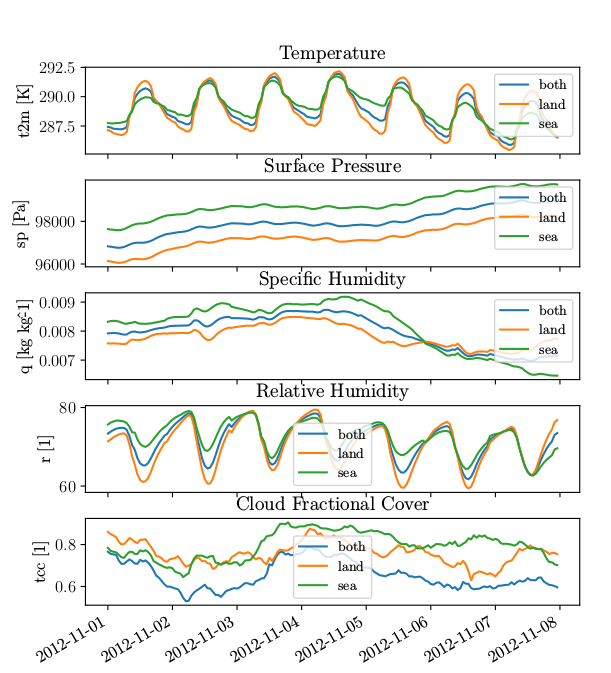
\includegraphics{python_figs/spatially_averaged_one_week_from_2012-11-01.png}
    \caption{\acrshort{ecc} variables first week November 2012.}
    \label{fig:nov12}
\end{figure}
\begin{figure}[ht]
    \centering
    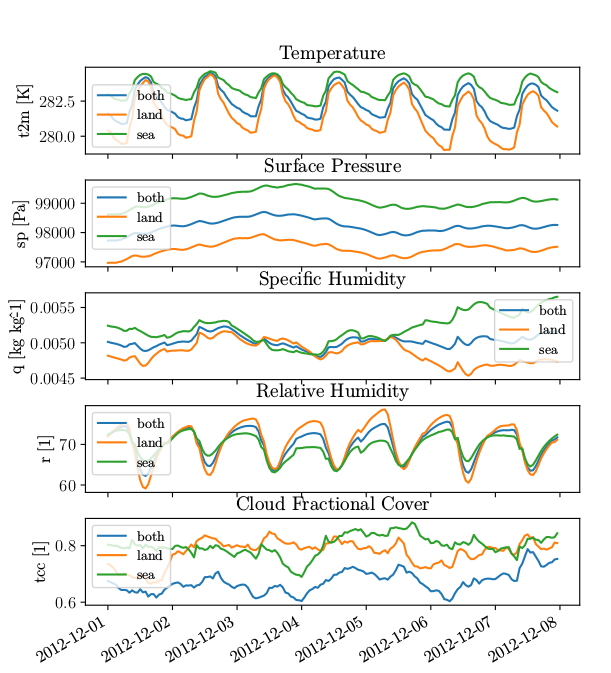
\includegraphics{python_figs/spatially_averaged_one_week_from_2012-12-01.png}
    \caption{\acrshort{ecc} variables first week December 2012.}
    \label{fig:dec12}
\end{figure}

\cleardoublepage
\chapter{List of non-trainable architectures} \label{app:list_non_trainable_architectures}
%As a reference to future studies below is a listing of non-trainable architectures.
\begin{enumerate}
    \item $ConvLSTM-B_{10}-SL_{24}-128-3\times3$
    \item $ConvLSTM-B_{10}-SL_{24}-128-3\times3-32-3\times3$
    \item $ConvLSTM-B_{10}-SL_{24}-64-3\times3-64-3\times3$
    \item $ConvLSTM-B_{5}-SL_{24}-256-3\times3-256-3\times3$
    \item $ConvLSTM-B_{5}-SL_{6}-256-3\times3-256-3\times3$
\end{enumerate}

%\textbf{List of models trained to slow, will be finished in 6 days. \textbf{Double check config.}}
%\begin{enumerate}
%    \item $ConvLSTM-B_{5}-SL_{6}-256-3\times3$
%    \item $ConvLSTM-B_{5}-SL_{6}-256-1\times1$
%\end{enumerate}
\cleardoublepage
\section{Performance of AR-models} \label{app:mae_plots}
\begin{figure}[ht]
    \centering
    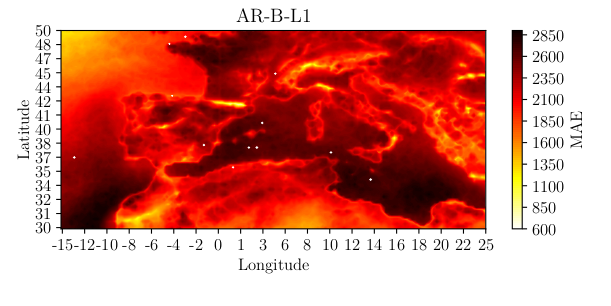
\includegraphics{python_figs/mea_best_ar_model_tcc_L1_in_folder_AR-B-L1.png}
    \caption{\acrshort{mae} of model $AR-B-L_1$.}
    \label{fig:grid_mae_ARBL1}
\end{figure}
\begin{figure}[ht]
    \centering
        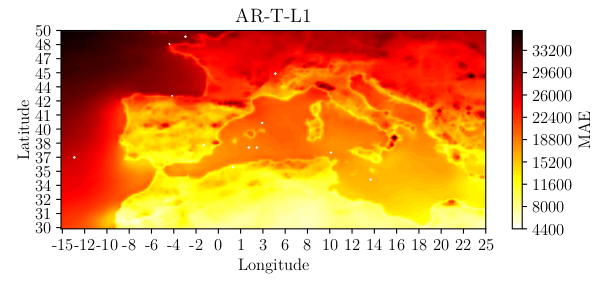
\includegraphics{python_figs/mea_best_ar_model_tcc_L1_in_folder_AR-T-L1.png}
    \caption{\acrshort{mae} of model $AR-T-L_1$.}
    \label{fig:grid_mae_AR-T-L1}
\end{figure}
\begin{figure}[ht]
    \centering
    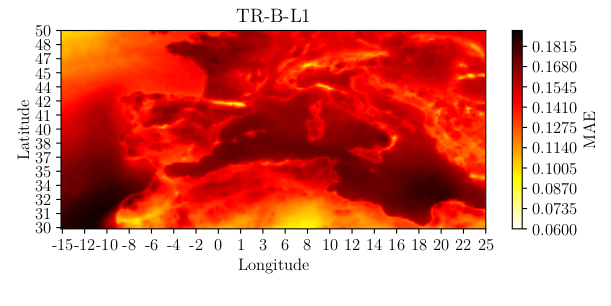
\includegraphics{python_figs/mea_best_ar_model_tcc_L1_in_folder_TR-B-L1.png}
    \caption{\acrshort{mae} of model $TR-B-L_1$.}
    \label{fig:grid_mae_TRBL1}
\end{figure}
\cleardoublepage
\chapter{Series of 24-hour Forecast} \label{app:pred_sequence}
\begin{figure}[ht]
    \centering
    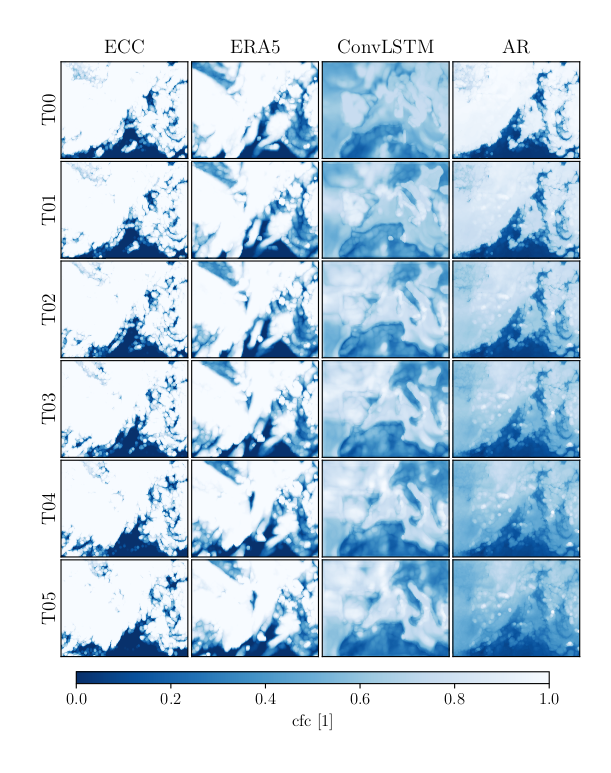
\includegraphics{python_figs/comparing_seq_part_1_of4_jan2.png}
    \caption{Hours zero to five of the forecast.}
    \label{fig:part1/4}
\end{figure}
\begin{figure}[ht]
    \centering
    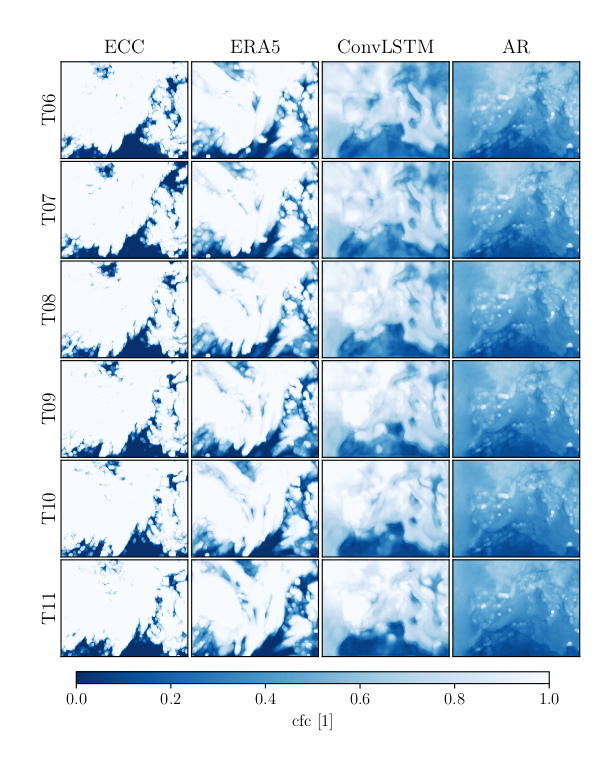
\includegraphics{python_figs/comparing_seq_part_2_of4_jan2.png}
    \caption{Hours six to 11 of the forecast.}
    \label{fig:part2/4}
\end{figure}
\begin{figure}[ht]
    \centering
    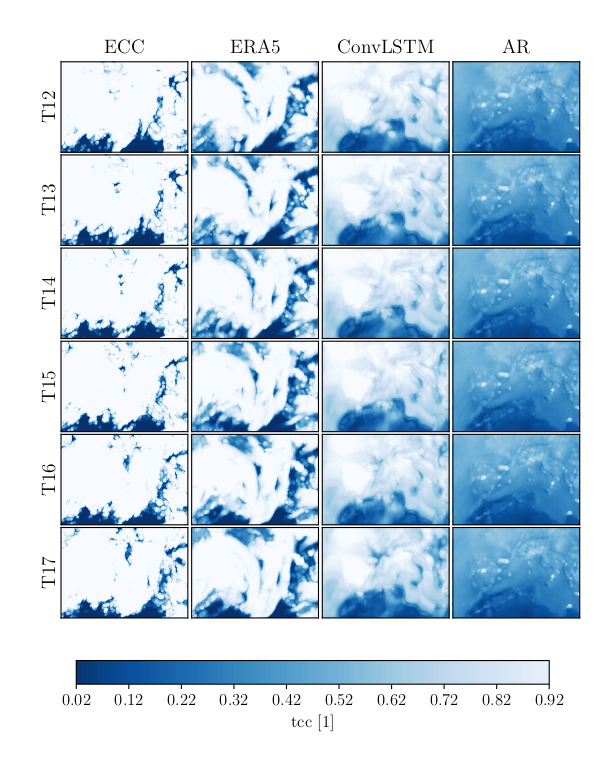
\includegraphics{python_figs/comparing_seq_part_3_of4_jan2.png}
    \caption{Hours 12 to 17 of the forecast.}
    \label{fig:part3/4}
\end{figure}
\begin{figure}[ht]
    \centering
    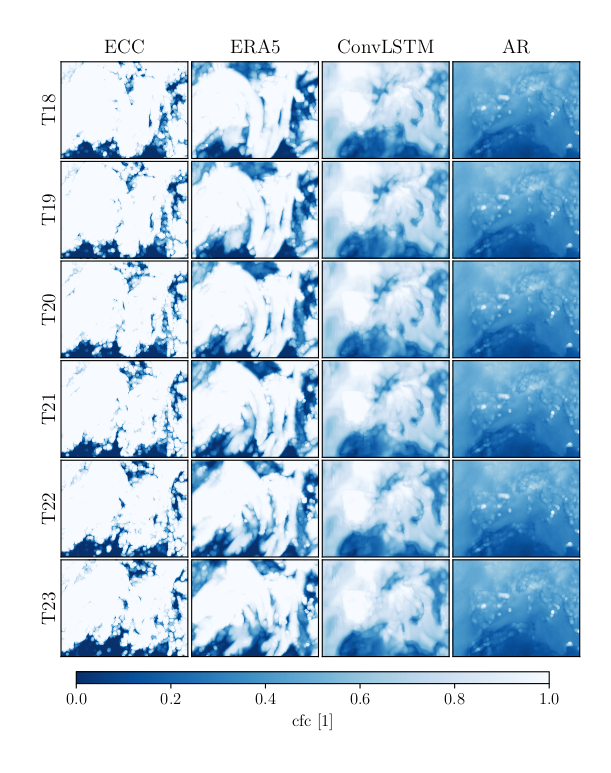
\includegraphics{python_figs/comparing_seq_part_4_of4_jan2.png}
    \caption{Hours 18 to 23 of the forecast.}
    \label{fig:part4/4}
\end{figure}
\cleardoublepage
\chapter{24-hour Forecasts}
\begin{figure}[ht]
    \centering
    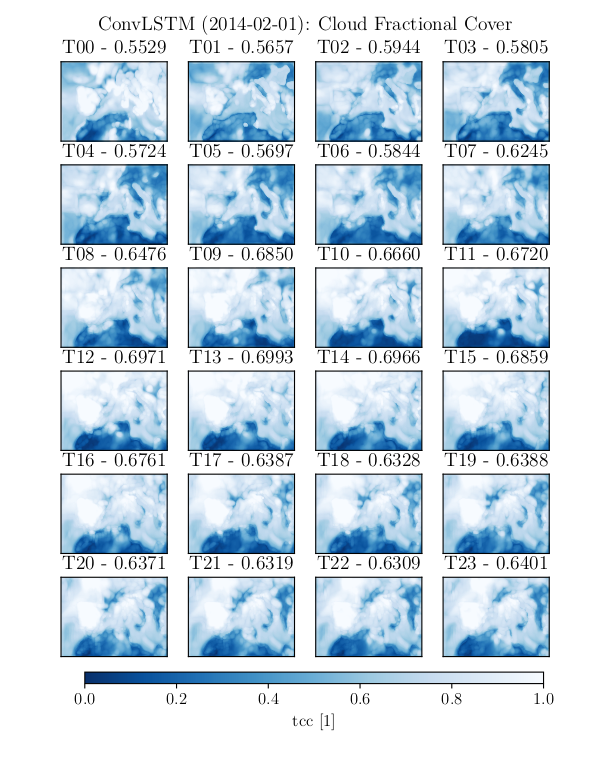
\includegraphics{python_figs/timelapse_convlstm_24hrs_from_2014-02-01.png}
    \caption{Cloud cover forecast produced by $ConvLSTM-B_{10}-SL_{24}-32-3\times3-32-3\times3$. Initiated on January 2, 2014.The area mean cloud fraction is included in the title.}
    \label{fig:timelapse_3x3}
\end{figure}
\begin{figure}[ht]
    \centering
    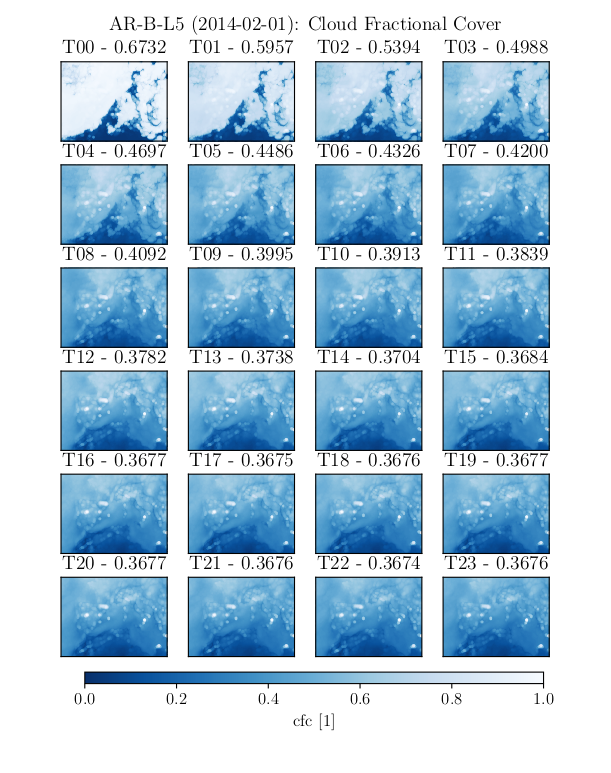
\includegraphics{python_figs/AR-B-L5_timelapse_cloud_cover_24hrs_from_2014_02_01.png}
    \caption{24 hour cloud cover forecast produced by $AR-B-L1$.  Initiated on January 2, 2014. The area mean cloud fraction is included in the title.}
    \label{fig:timelapse_ar}
\end{figure}
\begin{figure}[ht]
    \centering
    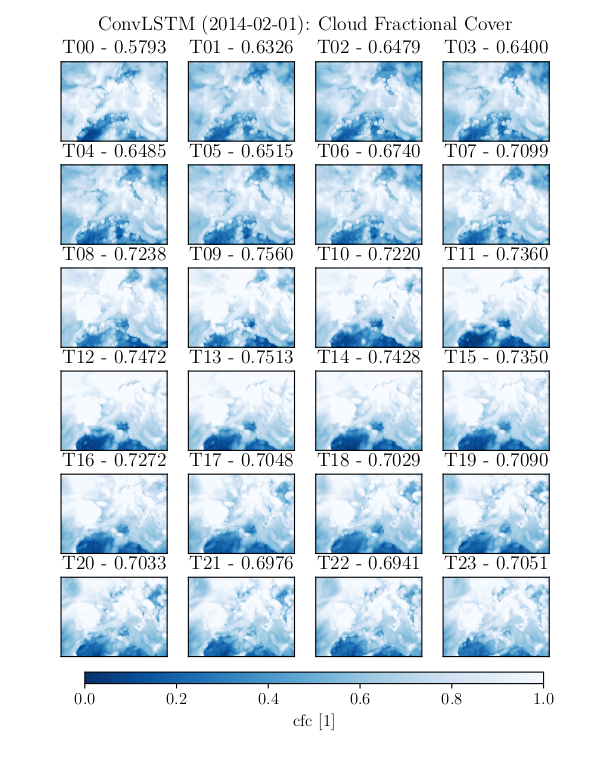
\includegraphics{python_figs/timelapse_convlstm_1x1_24hrs_from_2014-02-01.png}
    \caption{Cloud cover forecast produced by $ConvLSTM-B_{10}-SL_{24}-32-1\times1-32-1\times1$. Initiated on January 2, 2014. The area mean cloud fraction is included in the title.}
    \label{fig:timelapse_1x1}
\end{figure}
\cleardoublepage
%%%%%%%%%%%%%%%%%%%%%%%%%%%%%%%%%%%%% signal artefact should be redefined if used
%\chapter{Miscellaneous} \label{app:misc}
%\begin{figure}[ht]
%    \centering
%    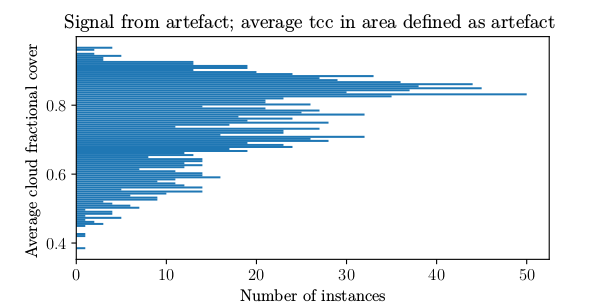
\includegraphics{python_figs/signal_artefact.png}
%\caption{Occurrence of artifact in \acrshort{ecc}.}
%    \label{fig:signal_artefact}
%\end{figure}

